\documentclass[twoside]{article}

\usepackage{aistats2023}

% If your paper is accepted, change the options for the package
% aistats2023 as follows:
%
%\usepackage[accepted]{aistats2023}
%
% This option will print headings for the title of your paper and
% headings for the authors names, plus a copyright note at the end of
% the first column of the first page.

% If you set papersize explicitly, activate the following three lines:
%\special{papersize = 8.5in, 11in}
%\setlength{\pdfpageheight}{11in}
%\setlength{\pdfpagewidth}{8.5in}

% If you use natbib package, activate the following three lines:
%\usepackage[round]{natbib}
%\renewcommand{\bibname}{References}
%\renewcommand{\bibsection}{\subsubsection*{\bibname}}

% If you use BibTeX in apalike style, activate the following line:
%\bibliographystyle{apalike}
%% TODO make pdg.sty file that allows you to import all PDG macros.
%%%%%%%%%%


\relax % Writing Tools
    \newcommand{\TODO}[1][INCOMPLETE]{{\color{red}\hangindent=0.5cm\rightskip=0.8cm$\smash{\Big\langle}$~\texttt{#1}~\raisebox{-0.3ex}{${\Big\rangle}$}\hspace{-1.5cm}\par}}


\relax
	\DeclareMathOperator*{\argmin}{arg\,min}
	\newcommand{\bundle}{\mathbin{+}}
    \newcommand{\Rext}{\mskip1mu\overline{\mskip-1mu\mathbb R\!}\,}

\relax
    %% Narrowing
    \usepackage{keyval}
    \makeatletter
    \define@key{setpar}{left}[0pt]{\leftmargin=#1}
    \define@key{setpar}{right}[0pt]{\rightmargin=#1}
    \define@key{setpar}{both}{\leftmargin=#1\relax\rightmargin=#1}
    \makeatother

    \newenvironment{narrow}[1][]
      {\list{}{\setkeys{setpar}{left,right}%
         \setkeys{setpar}{#1}%
         \listparindent=\parindent
         \topsep=0pt
         \partopsep=0pt
         \parsep=\parskip}\item\relax\hspace*{\listparindent}\ignorespaces}
      {\endlist}
    % \newenvironment{abstract}
    %     {\narrow[both=1in]\small}         
    %     {\endnarrow}


\relax % Bibliography
    \usepackage[backend=biber, style=authoryear]{biblatex}
    % \usepackage[backend=biber,style=authoryear,hyperref=true]{biblatex}
    \addbibresource{refs.bib}

    \DeclareLanguageMapping{american}{american-apa}
    % \renewcommand*{\nameyeardelim}{\addcomma\space}
    \DeclareDelimFormat{nameyeardelim}{\addcomma\space}
    % \listfiles

    \DeclareFieldFormat{citehyperref}{%
      \DeclareFieldAlias{bibhyperref}{noformat}% Avoid nested links
      \bibhyperref{#1}}

    \DeclareFieldFormat{textcitehyperref}{%
      \DeclareFieldAlias{bibhyperref}{noformat}% Avoid nested links
      \bibhyperref{%
        #1%
        \ifbool{cbx:parens}
          {\bibcloseparen\global\boolfalse{cbx:parens}}
          {}}}

    \savebibmacro{cite}
    \savebibmacro{textcite}

    \renewbibmacro*{cite}{%
      \printtext[citehyperref]{%
        \restorebibmacro{cite}%
        \usebibmacro{cite}}}

    \renewbibmacro*{textcite}{%
      \ifboolexpr{
        ( not test {\iffieldundef{prenote}} and
          test {\ifnumequal{\value{citecount}}{1}} )
        or
        ( not test {\iffieldundef{postnote}} and
          test {\ifnumequal{\value{citecount}}{\value{citetotal}}} )
      }
        {\DeclareFieldAlias{textcitehyperref}{noformat}}
        {}%
      \printtext[textcitehyperref]{%
        \restorebibmacro{textcite}%
        \usebibmacro{textcite}}}


\usepackage{tikz}
	\usetikzlibrary{positioning,fit,calc, decorations, arrows, shapes, shapes.geometric}
	\usetikzlibrary{cd}

	%%%%%%%%%%%%
	\tikzset{AmpRep/.style={ampersand replacement=\&}}
	\tikzset{center base/.style={baseline={([yshift=-.8ex]current bounding box.center)}}}
	\tikzset{paperfig/.style={center base,scale=0.9, every node/.style={transform shape}}}

	% Node Stylings
	\tikzset{dpadded/.style={rounded corners=2, inner sep=0.7em, draw, outer sep=0.3em, fill={black!50}, fill opacity=0.08, text opacity=1}}
	\tikzset{dpad0/.style={outer sep=0.05em, inner sep=0.3em, draw=gray!75, rounded corners=4, fill=black!08, fill opacity=1, align=center}}
	\tikzset{dpadinline/.style={outer sep=0.05em, inner sep=2.5pt, rounded corners=2.5pt, draw=gray!75, fill=black!08, fill opacity=1, align=center, font=\small}}

 	\tikzset{dpad/.style args={#1}{every matrix/.append style={nodes={dpadded, #1}}}}
	\tikzset{light pad/.style={outer sep=0.2em, inner sep=0.5em, draw=gray!50}}

	\tikzset{arr/.style={draw, ->, thick, shorten <=3pt, shorten >=3pt}}
	\tikzset{arr0/.style={draw, ->, thick, shorten <=0pt, shorten >=0pt}}
	\tikzset{arr1/.style={draw, ->, thick, shorten <=1pt, shorten >=1pt}}
	\tikzset{arr2/.style={draw, ->, thick, shorten <=2pt, shorten >=2pt}}

	\newcommand\cmergearr[5][]{
		\draw[arr, #1, -] (#2) -- (#5) -- (#3);
		\draw[arr, #1, shorten <=0] (#5) -- (#4);
		}
	\newcommand\mergearr[4][]{
		\coordinate (center-#2#3#4) at (barycentric cs:#2=1,#3=1,#4=1.2);
		\cmergearr[#1]{#2}{#3}{#4}{center-#2#3#4}
		}
	\newcommand\cunmergearr[5][]{
		\draw[arr, #1, -, shorten >=0] (#2) -- (#5);
		\draw[arr, #1, shorten <=0] (#5) -- (#3);
		\draw[arr, #1, shorten <=0] (#5) -- (#4);
		}
	\newcommand\unmergearr[4][]{
		\coordinate (center-#2#3#4) at (barycentric cs:#2=1.2,#3=1,#4=1);
		\cunmergearr[#1]{#2}{#3}{#4}{center-#2#3#4}
		}


\relax %% Double delimeters; I need this for pdg macros \aar and \bbr
    \newcommand{\nhphantom}[2]{\sbox0{\kern-2%
    \nulldelimiterspace$\left.\delimsize#1\vphantom{#2}\right.$}\hspace{-.97\wd0}}
    % \nulldelimiterspace$\left.\delimsize#1%
    % \vrule depth\dp#2 height \ht#2 width0pt\right.$}\hspace{-.97\wd0}}
    \makeatletter
    \newsavebox{\abcmycontentbox}
    \newcommand\DeclareDoubleDelim[5]{
    \DeclarePairedDelimiterXPP{#1}[1]%
        {% box must be saved in this pre code
            \sbox{\abcmycontentbox}{\ensuremath{##1}}%
        }{#2}{#5}{}%
        %%% Correct spacing, but doesn't work with externalize.
        % {\nhphantom{#3}{##1}\hspace{1.2pt}\delimsize#3\mathopen{}##1\mathclose{}\delimsize#4\hspace{1.2pt}\nhphantom{#4}{##1}}
        %%% Fast, but wrong spacing.
        % {\nhphantom{#3}{~}\hspace{1.2pt}\delimsize#3\mathopen{}##1\mathclose{}\delimsize#4\hspace{1.2pt}\nhphantom{#4}{~}}
        %%% with savebox.
        {%
            \nhphantom{#3}{\usebox\abcmycontentbox}%
            \hspace{1.2pt} \delimsize#3%
            \mathopen{}\usebox{\abcmycontentbox}\mathclose{}%
            \delimsize#4\hspace{1.2pt}%
            \nhphantom{#4}{\usebox\abcmycontentbox}%
        }%
    }
    \makeatother

\relax %%%%%%%%%   PDG  MACROS   %%%%%%%%
	\newcommand{\ssub}[1]{_{\!_{#1}\!}}
	
	% \newcommand{\bp}[1][L]{\mat{p}_{\!_{#1}\!}}
	% \newcommand{\bP}[1][L]{\mat{P}_{\!_{#1}\!}}
    \newcommand{\pdgunit}{\mathrlap{\mathit 1} \mspace{2.3mu}\mathit 1}
	
	\newcommand{\X}{\mathcal X}
	\newcommand{\V}{\mathcal V}
	\newcommand{\N}{\mathcal N}
	\newcommand{\Ed}{\mathcal E}
	\newcommand{\Ar}{\mathcal A}
	\newcommand{\ArST}{\hat\Ar}
	
    \newcommand{\balpha}{\boldsymbol\alpha}
    \newcommand{\bbeta}{\boldsymbol\beta}

	\newcommand{\bp}[1][L]{\mat{p}\ssub{#1}}
	\newcommand{\bP}[1][L]{\mat{P}\ssub{#1}}
	% \def\p_#1{p\ssub{#1}}
	\def\p_#1{\mathbb P_{#1}}	

	%%%%% a clever version of \Src,\Tgt, and \p that supresses subscripts
	\newif\ifsuba \subatrue
	\let\psimp\p  % \let\simpSrc\Src   \let\simpTgt\Tgt 
	% \renewcommand\Src[1]{\simpSrc{\ifsuba #1\fi}}
	% \renewcommand\Tgt[1]{\simpTgt{\ifsuba #1\fi}}
	\newcommand\Src[1]{\ifsuba S\mskip-2mu\vphantom{|}_{{#1}} \else S \fi}
	\newcommand\Tgt[1]{\ifsuba T\mskip-3mu\vphantom{|}_{{#1}} \else T \fi}
	% \def\p_#1(#2){\subafalse\psimp_{#1}(#2)\subatrue}

	% \newcommand\Src[1]{S\mskip-2mu\vphantom{|}_{{#1}}}
    % \newcommand\Tgt[1]{T\mskip-3mu\vphantom{|}_{{#1}}}	
    % \newcommand\Src[1]{X_{{#1}}}
    % \newcommand\Tgt[1]{Y_{{#1}}}
    % \newcommand{\Src}{\mathrm{Src}}
    % \newcommand{\Tgt}{\mathrm{Tgt}}
    % \newcommand\Src[1]{S\mskip-2mu\mathit{r\mskip-3muc}_{{#1}}}
    % \newcommand\Tgt[1]{T\mskip-5mu\mathit{g\mskip-1mut}_{{#1}}}
    % \newcommand\Src[1]{\mathsf{S}\mskip-2mu\vphantom{|}_{{#1}}}
    % \newcommand\Tgt[1]{\mathsf{T}\mskip-3mu\vphantom{|}_{{#1}}}
    

	\DeclareMathAlphabet{\mathdcal}{U}{dutchcal}{m}{n}
	\DeclareMathAlphabet{\mathbdcal}{U}{dutchcal}{b}{n}
	\newcommand{\dg}[1]{\mathbdcal{#1}}
	\newcommand{\PDGof}[1]{{\dg M}_{#1}}
	\newcommand{\UPDGof}[1]{{\dg N}_{#1}}
	\newcommand\VFE{\mathit{V\mkern-4mu F\mkern-4.5mu E}}

	\newcommand\Inc{\mathit{Inc}}
	\newcommand{\IDef}[1]{\mathit{IDef}_{\!#1}}
	\newcommand\OInc{\mathit{O\mskip-2.5muI\mskip-3.5mun\mskip-1.7muc}} % new version of Inc
	% \newcommand\CInc{\mathit{C\mskip-3.1muI\mskip-3.5mun\mskip-1.7muc}} % new version of IDef
	\newcommand\CDef{\mathit{C\mskip-3.5muD\mskip-2.5mue\mskip-1.5muf}} % new version of IDef
	% \newcommand{\SInc}{\mathit{S\mskip-1muI\mskip-1mun\mskip-1muc}} % new version of IDef
	% \newcommand{\ed}[3]{%
	% 	\mathchoice%
	% 	{#2\overset{\smash{\mskip-5mu\raisebox{-3pt}{${#1}$}}}{\xrightarrow{\hphantom{\scriptstyle {#1}}}} #3} %display style
	% 	{#2\overset{\smash{\mskip-5mu\raisebox{-3pt}{$\scriptstyle {#1}$}}}{\xrightarrow{\hphantom{\scriptstyle {#1}}}} #3}% text style
	% 	{#2\overset{\smash{\mskip-5mu\raisebox{-3pt}{$\scriptscriptstyle {#1}$}}}{\xrightarrow{\hphantom{\scriptscriptstyle {#1}}}} #3} %script style
	% 	{#2\overset{\smash{\mskip-5mu\raisebox{-3pt}{$\scriptscriptstyle {#1}$}}}{\xrightarrow{\hphantom{\scriptscriptstyle {#1}}}} #3}} %scriptscriptstyle
	\newcommand{\ed}[3]{#2%
	  \overset{\smash{\mskip-5mu\raisebox{-1pt}{$\scriptscriptstyle
	        #1$}}}{\rightarrow} #3}

	\newcommand{\bundle}{\mathbin{+}}
	\DeclareDoubleDelim
		\SD\{\{\}\}
	\DeclareDoubleDelim
		\bbr[[]]
	% \DeclareDoubleDelim
	% 	\aar\langle\langle\rangle\rangle
	\makeatletter
	\newsavebox{\aar@content}
	\newcommand\aar{\@ifstar\aar@one@star\aar@plain}
	\newcommand\aar@one@star{\@ifstar\aar@resize{\aar@plain*}}
	\newcommand\aar@resize[1]{\sbox{\aar@content}{#1}\scaleleftright[3.8ex]
		{\Biggl\langle\!\!\!\!\Biggl\langle}{\usebox{\aar@content}}
		{\Biggr\rangle\!\!\!\!\Biggr\rangle}}
	\DeclareDoubleDelim
		\aar@plain\langle\langle\rangle\rangle
	\makeatother


	% \DeclarePairedDelimiterX{\aar}[1]{\langle}{\rangle}
	% 	{\nhphantom{\langle}{#1}\hspace{1.2pt}\delimsize\langle\mathopen{}#1\mathclose{}\delimsize\rangle\hspace{1.2pt}\nhphantom{\rangle}{#1}}


% \author{$\{$Oliver E Richardson, Joseph Y Halpern, Christopher De Sa$\}$}

\begin{document}
% If your paper is accepted and the title of your paper is very long,
% the style will print as headings an error message. Use the following
% command to supply a shorter title of your paper so that it can be
% used as headings.
%
%\runningtitle{I use this title instead because the last one was very long}

% If your paper is accepted and the number of authors is large, the
% style will print as headings an error message. Use the following
% command to supply a shorter version of the authors names so that
% they can be used as headings (for example, use only the surnames)
%
%\runningauthor{Surname 1, Surname 2, Surname 3, ...., Surname n}

\twocolumn[

\aistatstitle{Inference in Probabilistic Dependency Graphs,\\
    via Exponential Cones and Otherwise}

\aistatsauthor{ Oliver E Richardson \And Joseph Y Halpern \And  Christopher De Sa }

% \aistatsaddress{ Institution 1 \And  Institution 2 \And Institution 3 } 
\aistatsaddress{Cornell University \And Cornell University \And Cornell University}
]

\begin{abstract}
    We provide the first tractable inference algorithm for Probabilistic Dependency Graphs (PDGs) with discrete variables, thereby placing PDGs on asymptotically similar footing as other graphical models, such as Bayesian Networks and Factor Graphs.
    This may be surprising, because PDGs are more expressive than other probabilistic graphical models, and also because a PDG inference algorithm can be used 
    % for ``inconsistency minimization'', 
    % which has been argued to be widely useful. 
    % to resolve inconsistencies, which has  as a generic modeling task. 
    % as a black box to train statistical models in ML.
    to calibrate a broad class of statistical models.
    
    The key to our approach is combining 
    (1) our finding that inference in PDGs with bounded tree-width can be reduced to a tractable linear optimization problem with exponential cone constraints,
    with (2) a recent interior point method that can (provably) solve such problems efficiently (Dahl \& Anderson, 2022).
    We provide a concrete implementation and emperical evaluation.
    In addition, we prove auxiliary results about complexity of this problem, and discuss other approaches to it. 
\end{abstract}




% \begin{narrow}
% %%-----------    A FRANK SUMMARY    ---------------
% Measuring / Estimating /  Inconsistency is very useful.
% For instance, (1) propogating it backwards through layers of computation = differentiable learning. 
% 
% Certain localized versions of it can be used to do other algorithms.

% How hard is it? 
% With interior point methods (convex programs with exponential cone constraints) we can do it in $O(n^4 \log n)$ time \& space, worst case for exact inference. So far, this means slightly harder than inference in Graphical models.
% \end{narrow}


% \tableofcontents

\section{INTRODUCTION}

Suppose you have a collection of probabilistic beliefs. 
Are they self-consistent? 
If not, how far off ar they from being consistent?
How much computation is necessary to synthesize these possibly-inconsistent into a single joint probability distribution?
% One way of viewing this paper is 
This paper may be viewed as providing partial answers---both theoretical and practical---to these questions.
% One way of viewing this paper  paper formalizes and partially answers to these questions.
% This paper may be veiwed as answering these questions.
% While this paper 
% it can also be read as addressing these deeper questions. 


% More concretely, we handle
Probabilistic Dependency Graphs, or pdgs \parencite{pdg-aaai},
are a particularly flexible class of probabilistic graphical models, which subsumes Bayesian Networks (BNs) and Markov Random Fields (MRFs).
The primary force behind the expressiveness of pdgs is their ability to capture inconsistent beliefs, and the natural way of measuring the degree of this inconsistency that the formalism provides.
%
Beyond its role in undergirding the semantics of pdgs, 
this inconsistency measurement also captures many standard
loss functions and statistical divergences, in the appropriate contexts
% Diagrammatic Calculus.
 \parencite{one-true-loss}.
% All of this paints a story of wanting 
It seems that in a  minimizing inconsistency is a 
generically useful modeling task. 

From a pragmatic point of view, though, PDGs are currently not yet very useful.
As it stands, they only have conceptual applications---one can use them to justify
a choice of loss function analytically, or to derive cute diagrammatic proofs
of inequalitites you likely already know \parencite{one-true-loss},
but it is impossible to compute with them.
% What use is a model without an inference algorithm? 
Until now, PDGs have been a model without an inference algorithm. 

We analyze the complexity of inference and updating in pdgs, and show that it is equivalent to inconsistency minimization.
Then, we reduce the problem to a linear program with exponenital cones constraints.
We then use a powerful recent interior point method
that can solve such problems in polynomial time \parencite{dahl2022primal}. 
% We then lean heavily on recent work 
% \parencite{dahl2022primal} showing that 
% such problems can be 
We provide a python implementation of our reduction, 
and also several generic optimization baselines, and then 
show that this exponential-cone-based approach is more precise
and, in some cases, faster than optimization baselines.
However, this approach that our algorithms are not as fast as exact inference methods for existing graphical models, such as beleif propogation.
% However, their asymptotics are not much worse.

\section{PRELIMINARIES}

\textbf{Basic notation.}
% This paper concerns the 
Let $\mat 1$ denote the all-ones vector.

{\color{red}\tt
TODO: unexplained notation / concepts
\begin{enumerate}[nosep]
\raggedright
\item tensor product $\otimes$
\item relative entropy $\kldiv\mu\nu$, conditional entropy $\H(Y|X)$
\item jusxtaposition of variables to make new variables, e.g., $XY$ is a variable.
\item PDG unions via $+$
\item Extended reals $\Rext := \mathbb R \cup \{\infty\}$
\item Tree width
\end{enumerate}
}


We write $\Delta S$ to denote the set of proability distributions over a finite set $S$.
Every variable $X$ can take on a finite set $\V(X)$ of possible values. 
% If $S$ is a finite set, we write $\Delta S$ for the set of probability distributions over $S$, i.e., the simplex over its elements. 
A conditional probability distribution (cpd) $p(Y|X)$ is a map 
$p : \V(X) \to \Delta \V(Y)$, so it assigns, to every $x \in \V(X)$, a probability distribution $p(Y|x) \in \Delta Y$, which is shorthand for $p(Y|X\!\!=\!x)$.
Given a joint distribution $\mu$ over many variables including both $X$ and $Y$, 
we write $\mu(X)$ for its marginal distribution on $X$, and $\mu(Y|X)$ for the cpd obtained by first conditioning on $X$ and then marginalizing to $Y$. 

% \textbf{Graph Theory.}

\textbf{Probabilistic Dependency Graphs.}
% \textbf{PDGs.}
We now give a quick overview of the PDG formalism,
following the more carefully motivated
expositions of \textcite{pdg-aaai,one-true-loss}.
%
% Let $\N$ be a set of variables, and 
%
% Fix a set $\N$ of variables. 
A probabilistic dependency graph (pdg) is just a collection of cpds, weighted by two kinds of confidence. More precisely:

\begin{defn}
    a pdg $\dg M
     % = (\mathcal P, \balpha, \bbeta)$ 
    $
    over $\N$ is a set $\Ed$ of edges, 
    each $L \in \Ed$ of which is associated with:
    \begin{itemize}[nosep]
        % \item (subsets of) variables $\Src L, \Tgt L \subset \N$, indicating the respective source and target variables of the edge;
        \item variables $\Src L, \Tgt L \in \N$, the source and target of $L$;
        \item a cpd $p\ssub L (\Tgt L | \Src L)$ on the target variables given the source variables,
        \item a weight $\beta\ssub L \in \Rext$ indicating 
            the modeler's confidence in the cpd $p\ssub L(\Tgt L | \Src L)$, and 
        \item a weight $\alpha\ssub L \in \mathbb R$ indicating 
            the modeler's confidence that the edge $L$ corresponds to an independent mechanism that determines $\Tgt L$ given $\Src L$. 
        \qedhere
    %     % \item $\mathcal P = \{ p\ssub L (\mat T_L | \mat S_L) \}_{L \in \Ed}$ is an indexed set of cpds   
    %     \item $\bbeta$ 
    \end{itemize}
\end{defn}

The incompatibility of a joint distribution $\mu(\N)$ over all variables, with such a PDG is given by a weighted sum of relative entropies:
\begin{align*}
    \Inc_{\dg M}(\mu) :=
        \sum_{L \in \Ed} \beta\ssub L\, \kldiv[\Big]{\mu(\Tgt L,\Src L)}{p\ssub L(\Tgt L | \Src L) \mu(\Src L)}.
        % \Ex_{\mu} \sum_{L \in \Ed} \beta\ssub L 
        %     \log \frac{\mu(\Tgt_L \mid \Src_L)}{p\ssub L(\Tgt_L \mid \Src_L)}
\end{align*}
$\Inc$ is called the ``quantitative'' term because it measures $\mu$'s discrepency
with the quantitative data in the cpds. 
Meanwhile, there is also a ``qualitative'' term, called the \emph{information deficiency}, given by
% \begin{align*}
$
    \IDef{\dg M}(\mu) := - \H(\mu) + \sum_{L \in \Ed} \alpha\ssub L\, \H_\mu(\Tgt L | \Src L).
$
% Although we won't motivate it here, 
which
    % , roughly speaking, 
    % is a generalization of maximum entropy that accounts for the
    % Seen from another angle, it
    models causal structure, and plays a significant role in allowing pdgs to capture (conditional) independencies.
Note that $\IDef{}$ does not depend on the cpds (``quantitative beliefs'') of $\dg M$, nor even the possible values of the variables---it is defined purely in terms of the topology of the graph and the weights $\balpha$. 
% \end{align*}
The PDG semantics are then given by a scoring fuction: 
$\bbr{\dg M}: \Delta \V\N \to \Rext$
the linear combination
\begin{align*}
    \bbr{\dg M}_\gamma(\mu) &:= \Inc_{\dg M}(\mu) + \gamma \IDef{\dg M}(\mu) 
        \numberthis\label{eqn:scoring-fn}
        \\
        =& \Ex_{\mu}\left[\, \sum_{L \in \Ed} \log \frac
            {\mu(\Tgt L| \Src L)^{\beta\ssub L - \gamma \alpha \ssub L}}
            {p\ssub L(\Tgt L | \Src L)^{\beta \ssub L}}
        \right] - \gamma \H(\mu)
        .
\end{align*}

The notation $\bbr{\dg M}^*_\gamma := \argmin_\mu \bbr{\dg M}_\gamma(\mu)$ denotes the set of optimal distributions at a particular $\gamma$.
Of particular interest is the ``quantitative limit'' as $\gamma \to 0$, 
at which there is a unique optimal joint distribution, $\bbr{\dg M}^*$.
This distribution uniquely achieves the smallest information deficiency among those distributions maximally compatible with $\dg M$. 

One should be careful to distinguish this joint distribution $\bbr{\dg M}^* \in \Delta\V \N$, which arises in the limit as $\gamma \to 0$, from $\bbr{\dg M}^*_0$, the set of distributions that minimize $\Inc_{\dg M}$ which contains $\bbr{\dg M}^*$, and possibly many others. 

The inconsistency of a PDG $\dg M$ is the smallest possible score of any distribution:
\begin{align*}
    \aar{\dg M}_\gamma := \inf_{\mu \in \Delta\!\V\!\N}\, \bbr{\dg M}_\gamma(\mu).
\end{align*}
To parallel the notation for scoring functions, when we omit the subscript, we refer to the limit as $\gamma\to 0$, which, unlike before, obeys $\aar{\dg M} = \aar{\dg M}_0$. 

\textbf{Exponential Cones.}
The exponential cone is the convex set
\begin{align*}
    K_{\mskip-1mu\exp} &:=\!\!\!\!\!\!
        \begin{aligned}
        \big\{ (x_1, x_2, x_3) &: 
                x_1 \ge x_2 e^{x_3 / x_2},\, x_2 > 0 \big\} 
        \\\quad \mathbin{\cup}\, \big\{ (x_1, 0, x_3) &: x_1 \ge 0,\, x_3 \le 0 \big\} 
    \end{aligned}
    \subset \mathbb R^3.
\end{align*}
% $K_{\exp}$ is non-symmetric, and cannot .
Recent work in interior point methods has
provided a way to solve linear optimization problems with such constraints in polynomial time \parencite{dahl2022primal},
provided that $x_1, x_2$ and $x_3$ are affine transformations of the program variables. 

% \TODO[Should I talk about disciplined convex programming here? 
%     It might go something like this:]
% 
% In the discipline c
% Exponential cone constraints constraints of the form $(a,b,c) \in K_{\exp}$ may be added to convex programs, so long as $a,b,$ and $c$ are affine transformations of the program variables. 


\section{UPDATING AND INFERENCE VIA INCONSISTENCY MINIMIZATION}
    \label{sec:inf-via-inc}

We are now equiped to talk more technically about inference in PDGs. 
Since PDG semantics are already given in terms of a scoring function,
the obvious thing to do is to find a distribution that minimizes it. 
% There are some immediate 
There are several immediate difficulties.
% We immediately run into some obstacles.
% There are some obstacles to this.


\begin{enumerate}[nosep, label=\textbf{D\arabic*.}]
    \item Even writing down a distribution $\mu$, let alone evaluating its score $\bbr{\dg M}_\gamma (\mu)$, or minimizing it, takes exponential time.
    
    \item Generally speaking, optimization is computationally difficult.
        Even our most powerful optimization techniques only provably find optima in certain special cases.
    Unfortunately, while standard optimization techniques seem to work in practice
    (more-or-less; see \cref{sec:expts}), the standard theoretical tools do not apply in our setting. 
        % and even if it can be 
        Despite being strictly convex \parencite{pdg-aaai},
        and even $C^\infty$ smooth, 
        in general $\bbr{\dg M}_\gamma$ is neither Lipshitz nor self-concordant.
         % convex (in $\mu$, which is exponentially large),
        
    
    \item Even if we coulld easily find optimizers of the function $\bbr{\dg M}_\gamma$ for fixed $\gamma > 0$, it's still not obvious that this would allow us to calculate the unique limiting distribution $\bbr{\dg M}*$.
\end{enumerate}

We will ultimately address each of these issues, but before we do so, 
% let's start with a shift in perspective.
let's start by looking at the problem in a different way.


% We start with a shift in perspective, which .
% Rather than 
For a moment, let's take the persepctive taken in \textcite{one-true-loss},
in which we throw all of the relevant pieces in a PDG, and try to minimize inconsistency.
Well, we have a PDG $\dg M$, and we also have a candidate joint distribution $\mu$.
What if we put them both on the same footing, in a new PDG, and measure its inconsistency?
It is not hard to show that the distribution any distribution $\mu$ that minimizes this quantity must also satisfy $\mu \in \bbr{\dg M}_\gamma^*$. More generally, 

\begin{linked}{prop}{optimalYgivenX}
	% \label{prop:optimalYgivenX}
	% For all $\dg M$, $X,Y\in\N^{\dg M}$, and $\gamma > 0$, we have that
    For all variables $X,Y$, and $\gamma > 0$, 
	$$\displaystyle
		% \argmin_{p : X \to \Delta Y}
		\argmin_{p(Y|X)}\,
        \aar{\dg M + p}_\gamma =
		\Big\{ \mu(Y | X) :  \mu \in \bbr{\dg M}_\gamma^* \Big\}
	,$$
% \end{linked}
% 
% In the limit of small $\gamma$, since there is only one such distribution,
% the expression beomes simpler.
% 
% \begin{linked}{coro}{smallgammaopt}
and in the quantiative limit, 
	$\displaystyle
		\bbr{\dg M}^*(Y | X)
	$ is the unique minimizer of the function
$
    p(Y|X) \mapsto \aar{\dg M + p}
$
which includes a conditional probability on $Y$ given $X$ into the PDG $\dg M$. 
\end{linked}

Consequently, if we are only interested in querying the marginal probability of some small subset $Y$ of variables conditioned on other ones $X$ (i.e., the usual form of a query to a graphical model), and we had an efficient way to estimate the inconsistency of a guess $p(Y|X)$ with the rest of the model, we would have successfully cleared obstacle \textbf{D1}.
One might worry that this reformulation could increase the difficulty of optimization (\textbf{D2})---that we might lose the several nice properties we do have---but fortunately, this concern is not substantiated. 

\begin{linked}{prop}{smooth-and-strictly-cvx}
	The map $p \mapsto \aar{\dg M \bundle p}_\gamma$ is smooth and
		strictly convex 
        %for $\gamma$%
	% (concretely: all $\gamma$ less than $\min (\{1\}\cup\{ \beta^{\dg M}_L : L \in \Ed^{\dg M}\})$
    when $\gamma < \min \{1\} \cup \{\beta_L\}_{ L \in \Ed}$.
	% .
\end{linked}

Operationally, though, we still haven't made much progress, since
we still don't have an easy way to compute $\aar{ ~\cdot~ }_\gamma$. 
In \cref{sec:complexity}, we will see why.
For now, let's focus instead on addressing \textbf{D2} first, an approach
which will ultimately be more fruitful.
 
% \begin{linked}{prop}{sementics-via-inconsistency}
% 	$\displaystyle
% 		\bbr{\dg M}_\gamma(\mu)
% 			% =  \aar*{\dg M \bundle \mu!}_\gamma
%             =\aar[\Big]{\dg M \bundle \overset{(\beta: \infty)}\mu}_{\!\!\gamma}.
% 			% \qquad\Big(~= \lim_{t \to \infty} \aar[\Big]{\dg M \bundle \overset{(\beta:t)}\mu}_{\!\!\gamma}
% 			% 	~\Big)
% 	% \qquad\text{and}\qquad
% 	% \bbr{\dg M}(\\)
% 	$
% \end{linked}
% 
% So it seems that generic optimization algorithms will
% give us a foothold on inference.
% However, the PDG objective \eqref{eqn:scoring-fn} 

% \begin{prop}
% \begin
%     	% \label{prop:optimalYgivenX}
%     	% For all $\dg M$, $X,Y\in\N^{\dg M}$, and $\gamma > 0$, we have that
%     	$\displaystyle
%     		\argmin_{p : X \to \Delta Y} \aar{\dg M + p}_\gamma =
%     		\Big\{ \mu(Y | X) :  \mu \in \bbr{\dg M}_\gamma^* \Big\}
%     	$.
% \end{prop}

\section{REDUCTIONS TO CONVEX PROGRAMS WITH EXPONENTIAL CONE CONSTRAINTS}
    \label{sec:reductions}

We now present the central finding of our paper:  observation that the PDG objective $\bbr{\dg M}_\gamma$ can be written
as a linear optimization problem with exponential cone constraints.

We will proceed as follows: 
\begin{enumerate}[itemsep=0pt]
    \item
    illustrate how to find the minimizers of $\Inc$, in a simple setting with only one variable and no conditional distributions.
    \item
    show how the same approach can be generalized to find minimizers of $\Inc$ in general PDGs,
    \item \label{item:+idef}
    show how to find $\bbr{\dg M}^*$, the unique distribution specified by $\dg M$ in the quantitative limit.
    
    % \item \label{item:cccp}
    % employ the convex-concave procedure 
    % \parencite{yuille2003concave}, to find some minimizer $\mu^* \in \bbr{\dg M}^*_\gamma$ (although it may not be unique), for fixed $\gamma > 0$.
    % 
    \item 
    % Finally, show how \cref{item:+idef,item:cccp} can also be achieved 
    Finally, show how this can all be done
    with a more efficient compact representation, for PDGs that have
    bounded tree-width.
\end{enumerate}

\subsection{}\label{sec:illust}

To illustrate the idea, consider the special case in which our PDG contains only one variable $X$, which takes values $\V(X) = \{1, \ldots, n\}$. 
Suppose further that for every edge $j \in \Ed = \{1, \ldots, k\}$, the cpd $p_j(X)$ is an unconditional dsitribution over $X$. 
    % i.e., $\Tgt k = X$, and $\Src k = \emptyset$.
% Such unconditional probabilities may be identified with unit vectors $\mat p\ssub L \in \mathbb R^n$.  Similarly a candidate (``joint'') distribution $\mu(X)$
Such unconditional probabilities may be identified with unit vectors $\mat p_j \in \mathbb R^n$, and all $k$ of them may conjoined to form a stochastic matrix $\mat P = [\,p_{ij}] \in [0,1]^{n \times k}$.
Of course, a candidate (``joint'') distribution $\mu(X)$
may be represented as a unit vector $\mat m \in \mathbb R^n$. 
%
% Now, consider another collection of vectors $\{\mat t\ssub {\,L}\,\in \mathbb R^n\}_{L \in \Ed}$ and notice that:
% \begin{align*}
%     \forall  L &\in \Ed.~~ 
%     (-\mat t\ssub L\,, \mat m, \mat p\ssub L) \in K_{\exp}^n \\
%         &\iff 
%             \forall  L \in \Ed.~~
%             \mat t \succeq {\mat m} \log \frac{\mat m}{\mat p}
%         \\&\implies \sum_{L \in \Ed}\sum_{i=1}^n t_i  \ge \kldiv{\mat m}{\mat p}
% \end{align*}
Now consider a matrix $\mat U = [u_{ij}] \in \Rext^{n \times m}$,
and observe that:
\begin{align*}
    &(- \mat U,~ \mat m \otimes \mat 1,~ \mat P) \in K_{\exp}^{n \times k} \\
    &\iff \forall  i,j \in [n]\!\times\![k].~~ 
        (- u_{ij}, m_{i}, p_{ij}) \in K_{\exp} \\
    &\iff \forall  i,j \in [n]\!\times\![k].~~ 
            u_{ij} \ge m_i \log \frac{m_i}{p_{ij}} \\
    &\implies \forall j \in [n].~~  {\textstyle\sum_i} u_{ij}  \ge \kldiv{\mu}{p_j} \\
    &\implies \sum_{i,j} \beta_j u_{ij}  \ge \beta_j \kldiv{\mu}{p_j} \\
    &\iff \mat 1^{\sf T} \mat U \bbeta \ge \Inc(\mu)
    .
    % &\implies \sum_{L \in \Ed}\sum_{i=1}^n t_i  \ge \kldiv{\mat m}{\mat p}
\end{align*}

So now, if $(\mat U, \mat m)$ are a solution to the convex program
\begin{align*}
    \mathop{\text{\sf minimize}}
    % \min
    \limits_{\mat m, \mat T}~~
        \mat 1^{\sf T} \mat U \bbeta 
    \quad\text{\sf subject to}\quad &
        \mat 1^{\sf T} \mat m  = 1, \\[-2ex]
    % \begin{cases}
        (-\mat U,\;\, &\mat m\otimes \mat 1,\; \mat P) \in K_{\exp}^{n \times m},
    % \end{cases},
\end{align*}
then (a) the inconsistency $\aar{\dg M} = \mat 1^{\sf T} \mat U \bbeta$ equals the optimal objective value, and 
(b) $\mu \in \bbr{\dg M}^*_0$ is maximally compatible with $\mu$. 
% This illustrates the general principle, but 

\subsection{Adding More Variables, Conditionals, Marginals}

Having seen some of the details of the maxtrix computations, let's now move up a level, and identify finitely supported distributions with their simplex representations. 
% For example, we will implicitly identify a joint distribution $\mu$ 
% with the appropriate vector 
We now tackle the general case of a pdg 
$\dg M = (\N, \Ed, \mathcal P, \balpha, \bbeta)$.

For each $L \in \Ed$, let $N_L := |\V(\Src L, \Tgt L)|$ be the dimension of joint settings of the source and target values of $L$, i.e., the dimension of the cpd $p \ssub L$,
let $K := \sum_{L \in \Ed} N_L$ be the total dimension,
and let $\mat u = [u^L_{s,t}]^{L \in \Ed,}_{ (s,t) \in \V(\Src L, \Tgt L)}$
be a free variable in $\Rext^{K}$.
% of all of the condtional probabilities in $\dg M$.
% Let $t = (t^L)_{L \in \Ed} \in \Rext^{K}$.
{\color{red} Let $\Pi_{X}$ be the projection map that marginalizes to the variables $X$. }
%
Consider the problem
% \begin{align*}
%     % \min_{\mu, t} &\qquad
%     \min_{\mat m, \mat u} &\quad
%         % \Vert t \Vert_1  
%         \sum_{L}\beta_L\, | \mat u\ssub {\mskip 1muL}\mskip 1mu |
%     \\
%     \text{subject to:}&\;\;
%         % (-t^L, \mu(\Src L, \Tgt L), \mu(\Src L) p\ssub L(\Tgt L | \Src L)) 
%         % (-t^L, \Pi_{(\Src L \Tgt L)}\mu, \Pi_{(\Src L)} (\mu) p\ssub L(\Tgt L | \Src L)) 
%         \big(\!\shortminus\! \mat u\ssub L,~ \Pi_{\Src L\Tgt L}\!(\mat m),~
%             \mat P\!\ssub L (\Pi_{\Src L}\!(\mat m) \otimes \mat 1) \big) 
%         % (-t^L_{xy}, \mu(x,y), )
%             \in K_{\exp},\\
%         &\qquad 
%             % \mu \ge 0, ~~ | \mu | = 1.
%             \mat m \ge 0, ~~ | \mat m | = 1.
%             \numberthis\label{eq:joint-prob}
% \end{align*}
\begin{align*}
    % \min_{\mu, t} &\qquad
    % \mathop{\text{\sf minimize}}\limits_{\mat m, \mat u} &\quad
    \mathop{\text{\sf minimize}}\limits_{\mu, \mat u} &\quad
        % \Vert t \Vert_1  
        % \sum_{L}\beta_L\, | \mat u\ssub {\mskip 1muL}\mskip 1mu |
        \sum_{L \in \Ed}\beta_L \, \sum_{\mathrlap{s,t \in \V(\Src L, \Tgt L)}} u^L_{s,t}
    \numberthis\label{eq:joint-prob}\\
    \text{\sf subject to:}&\quad \mu \in \Delta\V\N, \\
        \forall L \in \Ed.~&(-\mat u^L, \mu(\Src L, \Tgt L), \mu(\Src L) p\ssub L(\Tgt L | \Src L)) \in K_{\exp}.
        % (-t^L, \Pi_{(\Src L \Tgt L)}\mu, \Pi_{(\Src L)} (\mu) p\ssub L(\Tgt L | \Src L)) 
        % \big(\!\shortminus\! \mat u\ssub L,~ \Pi_{\Src L\Tgt L}\!(\mat m),~
            % \mat P\!\ssub L (\Pi_{\Src L}\!(\mat m) \otimes \mat 1) \big) 
        % (-t^L_{xy}, \mu(x,y), )
            % \in K_{\exp},
            % \\
        % &\qquad
    % \color{red}\text{\sf subject to:}
    \\
    \color{red}\text{previously}&\color{red}
        % (-t^L, \mu(\Src L, \Tgt L), \mu(\Src L) p\ssub L(\Tgt L | \Src L)) 
        % (-t^L, \Pi_{(\Src L \Tgt L)}\mu, \Pi_{(\Src L)} (\mu) p\ssub L(\Tgt L | \Src L)) 
        \big(\!\shortminus\! \mat u\ssub L,~ \Pi_{\Src L\Tgt L}\!(\mat m),~
            \mat P\!\ssub L (\Pi_{\Src L}\!(\mat m) \otimes \mat 1) \big) 
        % (-t^L_{xy}, \mu(x,y), )
            \in K_{\exp},\\
        &\qquad \color{red}
            % \mu \ge 0, ~~ | \mu | = 1.
            \mat m \ge 0, ~~ | \mat m | = 1.
\end{align*}

% This convex program has $K+1$ constraints 
% \TODO[ I've rewritten this a couple times, and it's always pretty ugly.
%     One higher level question: should we convert this to a different form? 
%     The fact that we can even write constraints this way hinges on the fact
%     that the arguments to the exponential cone are
%     affine transformations of the program variables, which 
%     this presentation sweeps under the rug entirely.
%     \hfill ]

Note that the marginals $\mu(\Src L, \Tgt L)$ and $\mu(\Src L)$ are
linear functions of $\mu$'s simplex representation, as required.
Logic similar to that in \cref{sec:illust} gives yields: 
\begin{prop}
    % If $(\mu, t)$ are a solution to \eqref{eq:joint-prob}, then
    % $\mu \in \bbr{\dg M}_0^*$,
    % % i.e., is maximally compatible with $\dg M$, and
    % and
    % $\sum_{L}\beta_L |t^L| = \aar{\dg M}$.
    If $(\mu, \mat u)$ are a solution to \eqref{eq:joint-prob}, then
    $\mu \in \bbr{\dg M}_0^*$,
    and
    $%\displaystyle
        \sum_{L}\beta_L \sum_{s,t \in \V(\Src L, \Tgt L)} u^L_{s,t} = \aar{\dg M}$.
\end{prop}

This is a start, but what we were really after was the unique distribution
$\bbr{\dg M}^*$ that also minimizes $\IDef{\dg M}$.

\subsection{Incorporating IDef}
    \label{sec:also-idef}
% To do this second pass, we will need this second property
% As $\gamma \to 0$, the limit of $\bbr{\dg M}_\gamma$

So far, we have only found \emph{some} distribution that minimizes $\Inc$; 
we really wanted to find the unique distribution $\bbr{\dg M}^*$.
% Fortunately, this can be done by simply running a second optimization problem, 
It turns out that a solution to \eqref{eq:joint-prob}  to construct a second optimization problem of a similar size.
% To justify our approach, we will to prove two more results.
To justify our approach, we need a little more math. 
% First, a characterization of 
First, a characterization of the set $\bbr{\dg M}^*_0$ of distributions that are maximally compatible with $\dg M$. 

\begin{prop}\label{prop:marginonly}
	For any PDG $\dg M$, 
	the highest-compatibility distributions (the minimizers $\bbr{\dg M}_0^*$ of $\Inc_{\dg M}$) all have the same conditional probabilities along the edges of $\dg M$.   
	That is to say, if there is an edge $\ed LXY \in \Ed^{\dg M}$, and $\mu_1, \mu_2 \in \bbr{\dg M}_0^*$ are quantitatively optimal distributions, then $\mu_1(Y|X) = \mu_2(Y|X)$.  
\end{prop}

As a result, having already found one minimizer of $\Inc_{\dg M}$ via \eqref{eq:joint-prob}, it suffices to constrain distributions that have the same conditional marginals along the edges, and now optimize $\IDef{}$.%
    \footnote{
        Technically, to deal with the possibility that variables we are conditioning on might have probability zero, 
        we require that $\mu(X,Y)\nu(X) = \mu(X) \nu(X,Y)$, rather than 
        $\mu(Y|X) = \nu(Y|X)$.
    }

We now run into a second issue: IDef is not convex in $\mu$. 
Fortunately, when we constrain to distributions that optimize $\Inc$, 
% it equals another function that is. 
it is.
Moreover, this function can also be represented with exponential cones.

\begin{prop}\label{prop:idef-frozen}
If $\mu \in \bbr{\dg M}_0^*$, 
then
\vspace{-1ex}
\[
    \IDef{\dg M}(\mu) = 
        % \kldiv[\bigg]{\mu}{ \prod_{L \in \Ed} \nu(\Tgt L | \Src L) }
            % + K(\dg M)
        % \Ex_\mu 
        % \left[
        \sum_{\mathclap{ w \in \V(\N)} }
            % \log \frac{\mu}{\prod_{L \in \Ed} \nu(\Tgt L | \Src L)}
            \mu(\mskip-1mu w \mskip-1mu)
            \log  \bigg(
                \faktor{\mu(\mskip-1mu w\mskip-1mu )\,}{\,\prod_{L \in \Ed} \nu(\Tgt Lw | \Src Lw)^{\alpha\ssub L}}
            \bigg)
        % \right]
        ,
\]
where $\{ \nu(\Tgt L | \Src L ) \}_{L \in \Ed}$ are the
conditional marginals along the edges $\Ed$ 
shared by all distributions in $\bbr{\dg M}^*_0$,
(per \cref{prop:marginonly}).
% and $K(\dg M)$ does not depend on $\mu$. 
\end{prop}

Having already computed a solution to \eqref{eq:joint-prob},
the denominator of the expression in \cref{prop:idef-frozen}
is a constant; call it
\[
\boldsymbol\psi := \prod_{L \in \Ed} \nu(\Tgt Lw | \Src Lw)^{\alpha\ssub L}.
\] 
\begin{prop}
% A solution to % \eqref{eqn:joint+idef}
If $\nu \in \bbr{\dg M}_0^*$, then $\bbr{\dg M}^*$ is the unique value of
$\mu$ that can 
% e an optimum of
solve
the convex problem
\begin{align*}
    \mathop{\text{\sf minimize}}\limits_{\mu, \mat u} & \quad
        \sum_{w \in \V\N} u_w
        % |\,\mat u\,| 
        \numberthis\label{eqn:joint+idef}\\
    \text{\sf subject to} &\quad 
        (-\mat u,  \mu, \boldsymbol\psi) \in K_{\exp},~~ \mu \in \Delta\V\N, \\
            &\forall L \in \Ed.~~\mu(\Src L \Tgt L) \nu(\Src L) = \mu(\Src L) \nu(\Src L, \Tgt L).
\end{align*}
\end{prop}


% \begin{algorithm}
% \begin{algorithmic}
%     \State $X$
% \end{algorithmic}
% \end{algorithm}


% \footnote{Indeed, $K_{\exp}$ is sometimes called the ``relative entropy cone'' for this reason.} 


% \subsection{Tree Deomposition
% \subsection{A Polynomial Algorithm for the Case of Bounded Tree-Width}
\subsection{A Less Expensive Representation for PDGs with Small Tree-Width}
    \label{sec:clique-tree-expcone}

The first property that makes this possible is 

\begin{linked}[Markov Property for PDGs]{prop}{markov-property}
	% Suppose $\dg M_1$ and $\dg M_2$ are compatible PDGs, and let $\mathbf X$ denote the variables they have in common.
	% Then for all $\gamma > 0$, we have that
	% \[
	%  	\bbr{\dg M_1 \bundle \dg M_2}^*_\gamma
	% 		% \subset
	% 		~\models~
	% 	% \mathrm I( \N_1 ; \N_2 \mid \mathbf X)
	% 	\N_1 \mathbin{\bot\!\!\!\bot} \N_2 \mid \mat X
	% \]
	% That is: in every optimizing distribution, for any value of $\gamma$, the variables of $\dg M_1$ and the variables of $\dg M_2$ are conditionally independent given their shared variables $\mat X$.
	% Suppose $\dg M_1$ and $\dg M_2$ are value-compatible PDGs,
	% with respective sets of nodes $\mat X_1 := \N^{\dg M_1}$ and
	% $\mat X_2 := \N^{\dg M_2}$.
	Suppose $\dg M_1$ and $\dg M_2$, over respective sets of variables $\mat X_1$ and $\mat X_2$.
	 % and let $\mathbf X$ denote the variables they have in common.
	Then for all $\gamma > 0$, we have that
	\[
	 	\bbr{\dg M_1 \bundle \dg M_2}^*_\gamma
			% \subset
			~\models~
		% \mathrm I( \N_1 ; \N_2 \mid \mathbf X)
		% \N_1 \mathbin{\bot\!\!\!\bot} \N_2 \mid \mat X
		% \N^{\dg M_1} \mathbin{\bot\!\!\!\bot} \N^{\dg M_2} \mid \mat X
		\mat X_1 \mathbin{\bot\!\!\!\bot} \mat X_2 \mid \mat X_1 \cap \mat X_2.
	\]
	That is to say: in every optimal distribution $\mu^* \in \bbr{\dg M_1 \bundle \dg M_2}^*_\gamma$,
     % for some $\gamma>0$, 
    the variables of $\dg M_1$ and of $\dg M_2$ are conditionally independent given the variables they have in common.
\end{linked}

The major consequence of \cref{prop:markov-property} is that we only have to consider distributions $\mu$ that come from calibrated clique trees. 

\TODO[TODO: Describe the minimum spanning aborescence + Bethe decomposition that makes this work, + also how the IDef calculation can be done]

\section{THEORETICAL ANALYSIS: THE COMPLEXITY OF INFERENCE}
    \label{sec:complexity}

Since inference in other graphical models is already NP-hard, 
and the class of PDGs subsumes capture them, it should be no surprise 
that inference in PDGs is NP hard as well.
%
%
One might imagine that \emph{resolving} the inconsistency is the hard part,
    as opposed to noticing it. 
Might it easier to simply determine whether or not a PDG is inconsistent?
% With some wishful thinking, one might imagine it possible
Alas, it is not.
% this is not the case either.

\begin{linked}{prop}{consistent-NP-hard}\label{sharp-p-hard}
    \begin{enumerate}[nosep,label={\rm{(\alph*)}}]
    \item Deciding if $\dg M$ is consistent is NP-hard.
    \item Computing $\aar{\dg M}_\gamma$ is \#P-hard, for all $\gamma > 0$.
    \end{enumerate}
\end{linked}

After all, as we saw in \cref{sec:inf-via-inc}, it seems an oracle that tells you your degree of inconsistency can be combined with a convex optimization algorithm to determine marginals in a way that does not scale with the rest of the graph. 

\begin{conj}
    Inference in a PDG---that is, computing conditional marginals of $\bbr{\dg M}^*$---%
    and the computing inconsistency $\aar{\dg M}$ are equally difficult:
        there are polynomial-time reductions from each to the other.
\end{conj}

If we do not restrict to finite variables, then the problem is much worse.

\begin{linked}{conj}{incomputable}
    The problem of deciding whether a PDG whose variables take values in $\mathbb N$ is not computable.
\end{linked}

% Now, essentially all of this is true for  
Morally, everything we've said here already applies to other graphical models.

Indeed, given widely held hardness hypotheses, bounded tree-width is essentially the \emph{only} class of graphical model that admits polynomial-time inference \parencite{chandrasekaran2012complexity}.

\begin{linked}{theorem}{main}
    % For   O( 3 n * ((3n+m+1)^3 ) * log(√n / ϵ) )  =   O( n^4 log(n)  log(1 / ϵ) )
There is an algorithm that takes $O(n^4 \log n  \log \nf1\epsilon )$ time,
and finds a point $\epsilon$-close in residual norm to the optimal distribution
$\bbr{\dg M}^*$, where $n$ is the total number of parameters needed to cover a clique tree.
\end{linked}

\TODO[ Finding the optimal clique tree is NP-hard. 
    So how can we guarantee we won't get a bad clique tree (i.e., much wider than the tree-width), so as to guarantee polynomial time?
    Do we have to know the bound?
    I imagine there's a standard answer, because exactly the same issue 
    arises for other graphical models. 
    \hskip-1.1em ]

The proof relies almost entirely on the analysis of \textcite{badenbroek2021algorithm},
which certifies that the optimization algorithm 
proposed in \textcite{dahl2022primal} works in polynomial time. 

\begin{table}
    % Let $m$ denote the 
    \centering
    \begin{tabular}{ccc}
        \toprule
        & BP &  ExpCone \\\cmidrule(lr){2-3}
        Time & $O(m t)$ & $O( m^4 \log m )$ \\
        Memory  & $O(m + )$ {\color{red}??} & $O( m^2 )${\color{red}????}\\    \bottomrule
    \end{tabular}
    
    \TODO[fill this in properly]
    
    \caption{ }
\end{table}


\section{INFERENCE WHEN
    \texorpdfstring{$\boldsymbol\gamma \boldsymbol> \mat 0$}{gamma > 0},
    VIA THE CONVEX-CONCAVE PROCEDURE }

We have now given an algorithm that provably finds the distribution $\bbr{\dg M}^*$ in polynomial time. 
What about optimal distributions for fixed $\gamma > 0$.



To do this, we re-use our work in \cref{sec:reductions} employ the convex-concave procedure 
\parencite{yuille2003concave}. to find some minimizer $\mu^* \in \bbr{\dg M}^*_\gamma$ (although it may not be unique), for fixed $\gamma > 0$.

The PDG objective can be written as \parencite[Proposition 4.6]{pdg-aaai}
\begin{align*}
    \bbr{\dg M}_\gamma(\mu) = 
        -\gamma\H(\mu) + 
            \sum_{L \in \Ed}
                % \left[
                \beta\ssub L\, \Ex_\mu 
                    \log \frac1{p\ssub L(\Tgt L | \Src L)}
                % \right]
                \\
            + \sum_{L \in \Ed}
            (\gamma \alpha \ssub L - \beta\ssub L)
                \Ex_\mu \log \mu(\Tgt L | \Src L)
\end{align*}
The first line is the sum of a linear term and a convex one,
and each individual term on the second line is either convex or concave, depending on the sign of the quantity $\gamma \alpha\ssub L - \beta\ssub L$. 
Once we sort the terms in to convex terms $f(\mu)$ and concave terms $g(\mu)$, we can choose an initial guess $\mu_0$, and iteratively compute
%
\begin{align*}
    \mu_{t+1} &:= \argmin_{\mu} f(\mu) + (\mu - \mu_{t})^{\sf T}
        \nabla g(\mu)
\end{align*}

As we will see in \cref{sec:expts}, the aproach presented here section is 
not very fast, but it is guaranteed to make progress, since
\begin{align*}
    f(\mu_{t+1}) \le  f(\mu_t) + (\mu_t - \mu_{t})^{\sf T}
        \nabla g(\mu)
\end{align*}
and eventually find an optimum. 

The slightly trickier part is combining this with the clique tree representation of \cref{sec:clique-tree-expcone}
        
\section{OTHER APPROACHES TO PDG INFERENCE} \label{sec:other-inference}

\subsection{}
A stronger result than \cref{prop:markov-property} holds as well.
\begin{prop}\label{prop:same-set-dists}
    % For all $\gamma > 0$ and in the limit as $\gamma \to 0$, 
    Let $\Ed$ be a set of (hyper-)edges over $\N$. 
    For every PDG $\dg M$ over $\N$ with edges $\Ed$, every $\gamma > 0$, and every optimum $\mu^* \in \bbr{\dg M}_\gamma^*$ of $\dg M$'s scoring function at $\gamma$, 
    there is a factor graph $\Phi$ with factors along $\Ed$ such that $\Pr_\Phi = \mu^*$. 
\end{prop}

In other words: every distribution that a PDG can pick out as optimal (for any choice of $\gamma > 0$ and also in the limit as $\gamma \to 0$), can also be described as a factor graph with the same structure as that PDG.
How do we square this with the \citeauthor{pdg-aaai}'s claim that PDGs are more general than factor graphs?

% This may be surprising, given how \citeauthor{pdg-aaai} position their model as strictly more expressive than other graphical models, because it implies that the optimal distribution 
\TODO[TODO: answer this question.\\
    The short answer: PDGs still compose differently, and in a way that respects the meaning of the probabilities. And just because you can find a factor graph that would have given you the right distribution after the fact, doesn't mean you could have specified the component factors.]
% The answer is simply that 


\TODO[Also: don't get lost; figure out how to continue as below:]
\cref{prop:same-set-dists} suggests another approach to avoiding an exponential representation of $\mu$: given a PDG, fit a factor graph that has the same structure to it. 

\subsection{Approximate Inference}
\subsubsection{Relaxing the Marginal Polytope}
Just as it is possible to do belief propogation on cluster graphs that are not trees,
so too is it possible to apply 
\cref{alg:ip-expcone}

\subsubsection{Variational Approaches}

Because of the deep connection between variational approaches 
shown in \parencite{one-true-loss}, 



\section{IMPLEMENTATION} \label{sec:implementation}
\section{EMPERICAL EVALUATION} \label{sec:expts}

\begin{figure}
    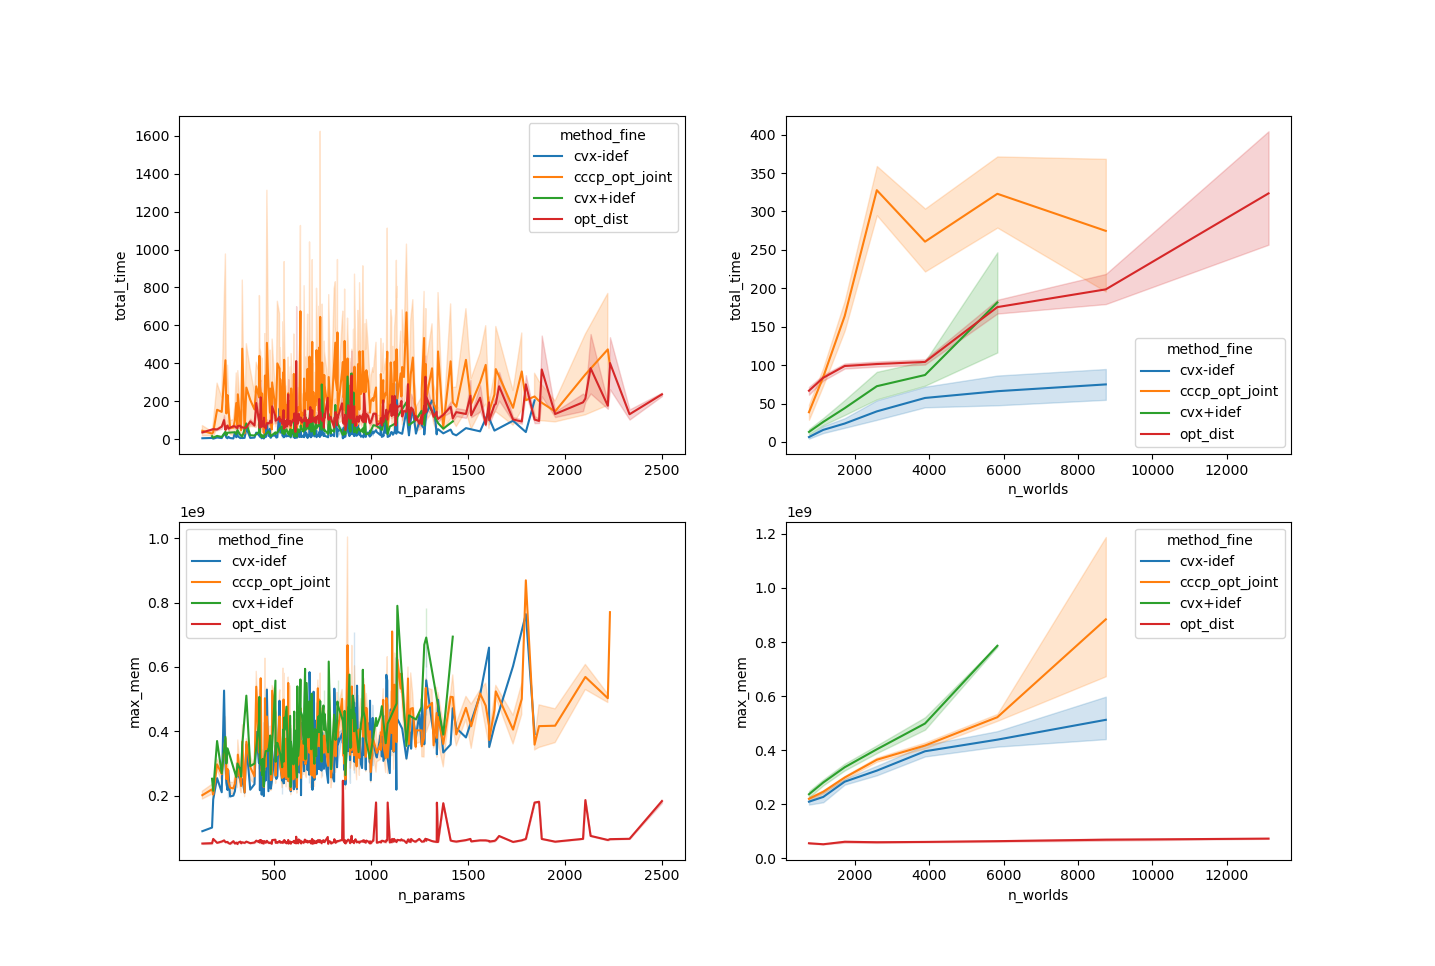
\includegraphics[width=\linewidth]{figs/resources-fine}
    \caption{
        The amount of resources: computation time (top) and maximum memory usage (bottom) for the various optimization methods (by color), as the size of the PDG increases, as measured by \texttt{n\_worlds} (right) and \texttt{n\_params} (left).
     }\label{fig:resources}
\end{figure}

\begin{figure}
    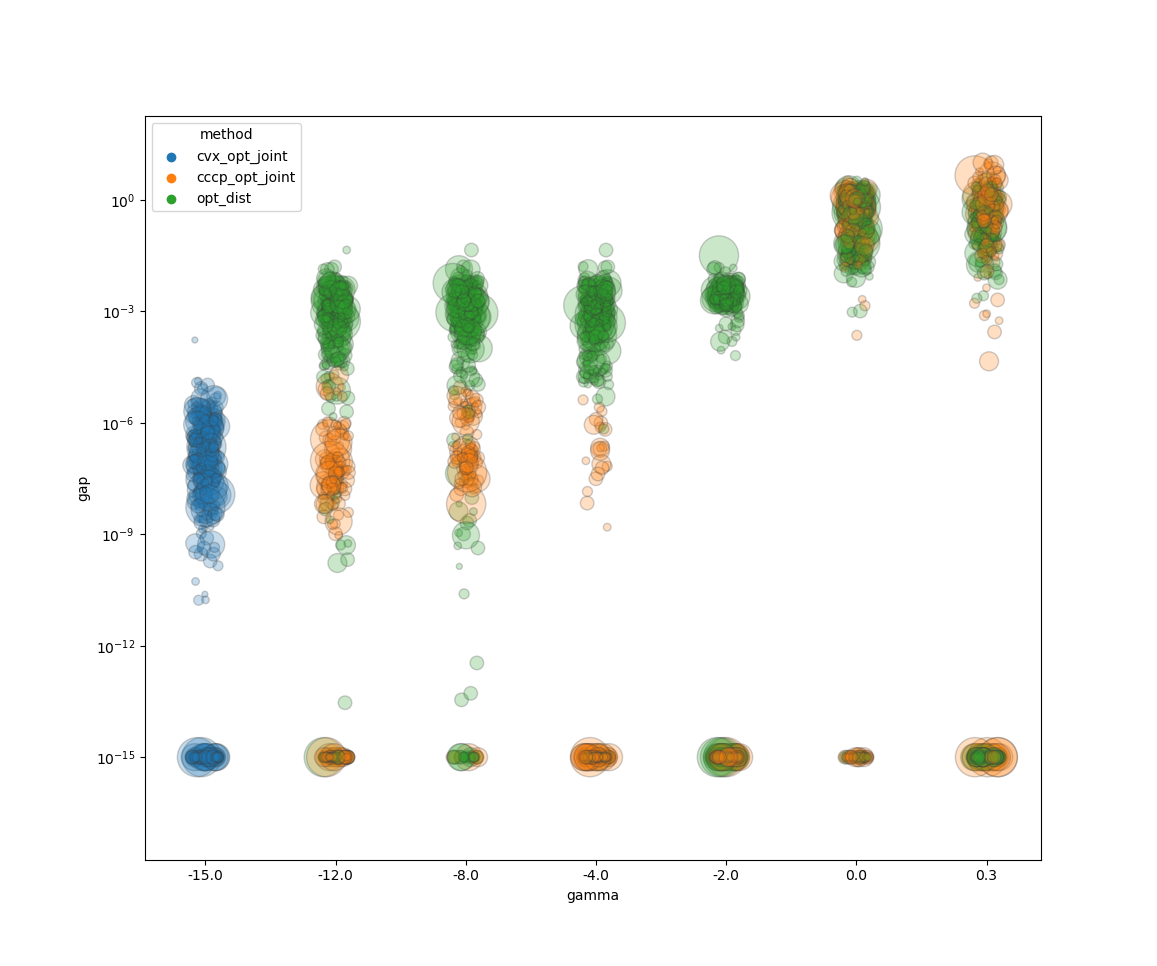
\includegraphics[width=\linewidth]{figs/gamma-vs-gap-bettergap}
    \caption{
        A graph of the gap (the difference between the attained objective value, and the best objective value obtained across all methods for that value of $\gamma$), 
        as $\gamma$ varies. As before, colors indicate method. 
        The size of the circle illustrates the relative number of worlds.
    }\label{fig:gamma-v-gap}
\end{figure}


\begin{figure}
    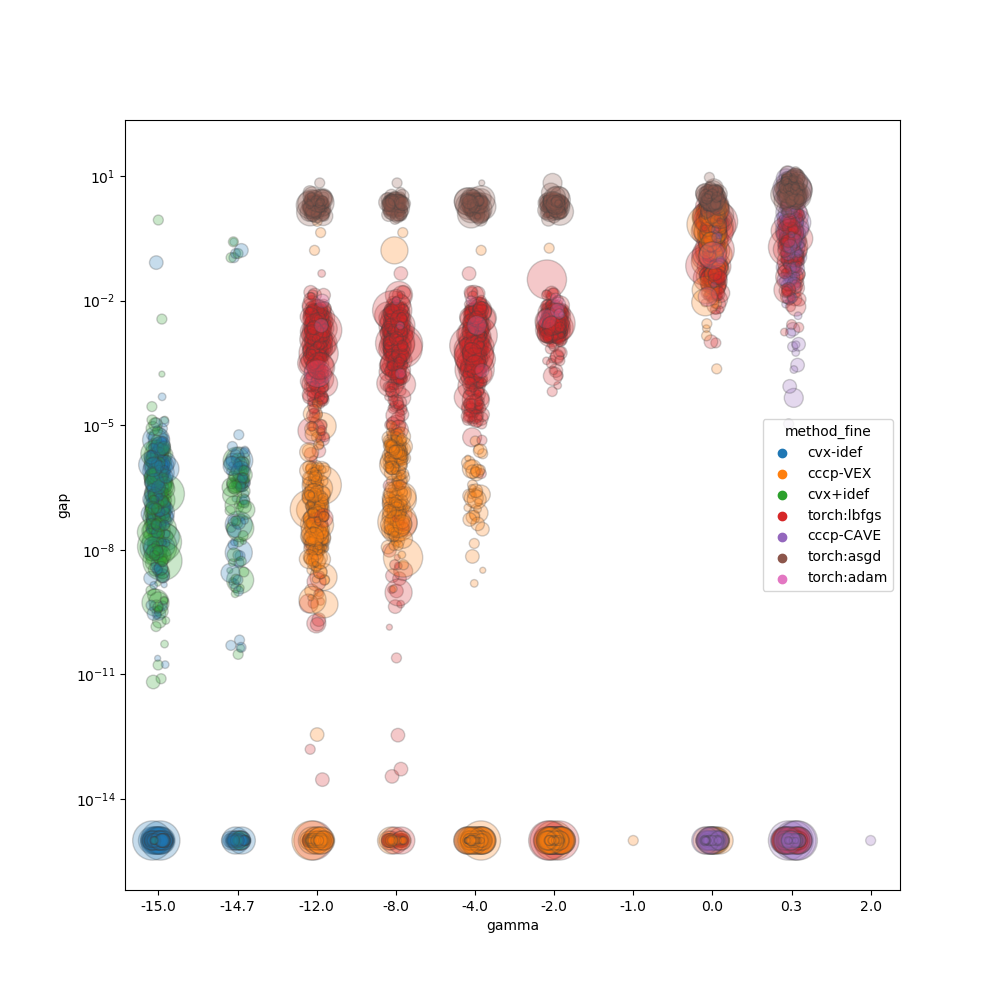
\includegraphics[width=\linewidth]{figs/2}
    \caption{
        A fine-grained variant of \cref{fig:gamma-v-gap}, which splits each method into sub-groups.
        The ExpCone methods \texttt{cvx\_opt\_joint} are split into two variants, depending on whether or not it also computed the second step described in \cref{sec:also-idef} to account for $\IDef{}$.
        The CCCP variants are \texttt{cccp\_opt\_joint} split into regimes where the entire problem is convex, and the entire problem is concave. The optimization approaches \texttt{opt\_dist} are split into three different optimizers: LBFGS, Adam, and accelerated Gradient Descent.
    }\label{fig:gamma-v-gap-fine}
\end{figure}

\begin{figure}
    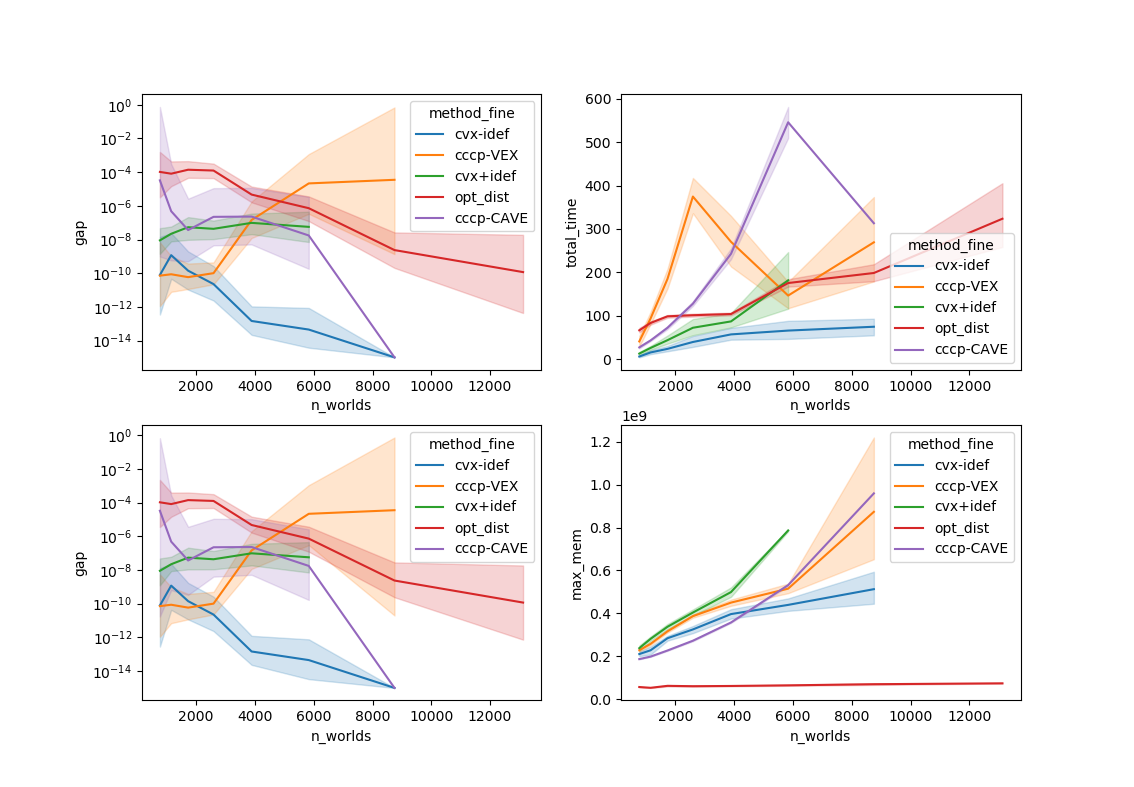
\includegraphics[width=\linewidth]{figs/1}
    \caption{
        A fine-grained variant of the right half of \cref{fig:resources}, 
        with gap information on the left. 
    }\label{fig:gap-resource-fine}
\end{figure}


\begin{figure}
    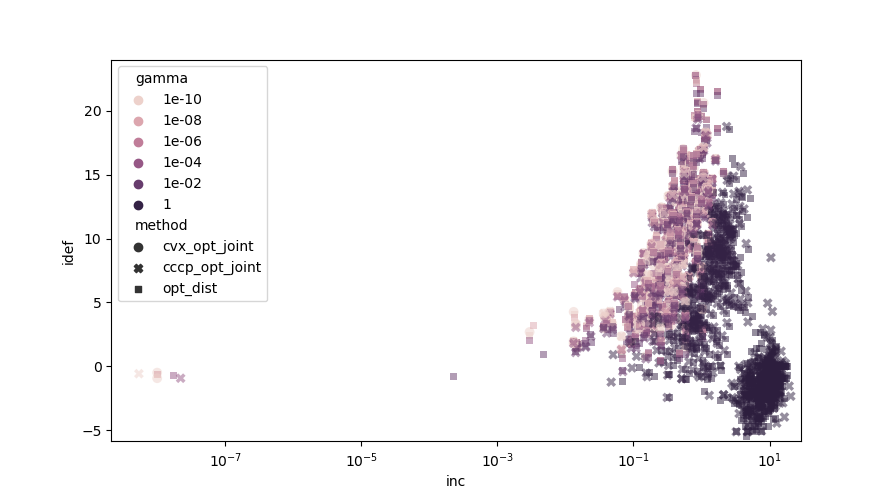
\includegraphics[width=\linewidth]{figs/inc-idef2}
    \caption{An illustration of the trade-off between $\Inc$ and $\IDef{}$. Darker collors correspond to larger $\gamma$.}\label{fig:inc-idef}
\end{figure}

\subsection{Comparison To Belief Propogation}

Since PDGs generalize other graphical models, one might wonder how our method stacks up against them. 
We benchmarked against the small networks, and some of the medium-sized ones, from the \href{https://www.bnlearn.com/bnrepository/}{\texttt{bnlearn}} repository. 



\subsection{Evaluations On Random PDGSs}
We start by focusing on emperical properties of the optimization over joint distributions.

We generated several hundred PDGs with various properties: 9 or 10 variables, each of which can take 2-3 values. Each PDG contains 7-15 hyper-edges, with 1-2 target nodes and 0-3 source nodes. The cpds are chosen by taking uniformly random numbers from [0,1] and normalizing appropriately, and every $\beta$ is set to 1.
For each PDG $\dg M$, we measure its complexity by:
\begin{itemize}[nosep]
    \item \texttt{n\_edges}, the number of edges in $\dg M$,
    \item \texttt{n\_params}, the total number of parameters across all the cpds of $\dg M$, and
    \item \texttt{n\_worlds}, the size of the joint distributions on the variables of $\dg M$.
\end{itemize}

\textbf{Capacity.} 
The black-box py-torch based approaches clearly have an edge in that they can handle larger models; see the cut-offs on the right sides of \cref{fig:resources,fig:gap-resource-fine}

\textbf{Resource Costs.} 
Look at \cref{fig:resources}. 
Note that the exponential cone methods without the CCCP (blue and green) are actually faster than LBFGS, which was the best-performing torch optimizer. 
However, they use \emph{significantly} more memory, and cannot handle more than 8000 worlds. 


\textbf{Accuracy.}
In addition to being faster, the exponential cone techniques are also more preicse.
Note that the CCCP is typically more precise than the black-box optimizers when the problem is fully convex $\gamma \le 1$, and mirrors the performance of the exp-cone algorithms for the quantitative limit on the left, in blue.  For combinations of larger $\gamma$ and more worlds however, the 20 iteration maximum we imposed is not nearly enough to get convergence, and the black-box optimizers are both faster and attain better objective values.

\section{DISCUSSION}

% Our anaysis 
Our analysis shows that inference in PDGs with bounded tree-width can be done .




\subsubsection*{Acknowledgements}
% All acknowledgments go at the end of the paper, including thanks to reviewers who gave useful comments, to colleagues who contributed to the ideas, and to funding agencies and corporate sponsors that provided financial support. 
% To preserve the anonymity, please include acknowledgments \emph{only} in the camera-ready papers.

\subsubsection*{References}
\printbibliography


\clearpage
\onecolumn
\appendix
\section{Proofs}

\recall{theorem:main}
\begin{lproof}\label{proof:main}
\end{lproof}

\subsection{}

\recall{prop:smooth-and-strictly-cvx}
\begin{lproof}\label{proof:smooth-and-strictly-cvx}
	% First, we deal with the convexity, for which we make use of \cref{lem:cvx2}.
	% \commentout{
	% 	\def\mw#1{{\mat w}_{\!_{#1}}}
	% 	\def\ofmw(#1|#2){(\mw{#1} | \mw{#2})}
	% 	\begin{align*}
	% 		\aar{\dg M \bundle p}_\gamma &= \inf_\mu \Big[ \Inc_{\dg M \bundle p}(\mu)
	% 			+ \IDef{\dg M \bundle p}(\mu) \Big] \\
	% 		&=  \inf_{\mu} \Ex_{\mat w \sim \mu}
	% 			\left[\log \mu(\mat w) +
	% 			 	\beta_p \log \frac{\mu\ofmw(Y|X)}{p\ofmw(Y|X)} \; +  \!\sum_{\ed LAB} \beta_L \log \frac{\mu\ofmw(B|A)}{\bp\ofmw(B|A)} + \alpha_L \log \frac{0}{\mu\ofmw(B|A)}\right] \\
	% 		&= f
	% 	\end{align*}
	% }
	We start by expanding the definitions, obtaining
	\begin{align*}
		\aar{\dg M \bundle p}_\gamma &= \inf_\mu ~\bbr{\dg M \bundle p}_\gamma(\mu) \\
			&= \inf_\mu \left[ \bbr{\dg M }_\gamma(\mu)
				+ \Ex_{x\sim\mu_{\!_X}} \kldiv[\Big]{\mu(Y\mid x)}{p(Y\mid x)} \right]\\
			&= \inf_\mu \left[ \bbr{\dg M }_\gamma(\mu)
				+  \kldiv[\Big]{\mu(X,Y)}{p(Y \mid X)\, \mu(X)} \right].
	\end{align*}
	% % Choose $\gamma < \min (\{1\}\cup\{ \beta^{\dg M}_L : L \in \Ed^{\dg M}\})$.
	% Since $\bbr{\dg M}_\gamma$ is a $\gamma$-strongly convex function of $\mu$ for all
	% such $\gamma < \min_L \beta_L$, and
	% $\kldiv{\mu_{XY}}{\mu_X \; p_{Y\mid X}}$ is 1-strongly
	% convex in $p$ for fixed $\mu$ (\cref{lem:Dstrongcvx}),
	% % $\thickD$ is convex in both of its arguments,
	% their sum is $\gamma$-strongly convex in $\mu$ and in $p$.
	% By \cref{lem:cvx2} taking an infemum preserves this convexity,
	% and so
	% $
	%  	\inf_\mu \left[ \bbr{\dg M }_\gamma(\mu)
	% 	+  \kldiv[\big]{\mu_{XY}}{p_{Y \mid X}\; \mu_X} \right]
	% $, which equals $\aar{\dg M \bundle p}_\gamma$,
	% is $\gamma$-strongly convex in $p$.
	% % $\aar{\dg M \bundle p}_\gamma$ is smooth
	% % Smoothness.


	% Choose $\gamma < \min (\{1\}\cup\{ \beta^{\dg M}_L : L \in \Ed^{\dg M}\})$.
	Fix $\gamma < \min_L \beta_L$. Then we know that $\bbr{\dg X}_\gamma(\mu)$ is a $\gamma$-strongly convex function for every PDG $\dg X$, and hence there is a unique joint distribution which minimizes it.

	\textbf{Strict Convexity.}
	Suppose $p_1(Y \mid X)$ and $p_2(Y\mid X)$ are two cpds on $Y$ given $X$.
	Fix $\lambda \in [0,1]$, and set $p_\lambda = (1-\lambda) p_1 + \lambda p_2$.
	Let $\mu_1, \mu_2$ and $\mu_\lambda$ be the joint distributions that minimze $\bbr{\dg M \bundle p_1}_\gamma$, $\bbr{\dg M \bundle p_2}_\gamma$ and $\bbr{\dg M \bundle p_\lambda}_\gamma$, respectively.  Then we have
	\begin{equation*}
		\aar{\dg M \bundle p_\lambda}_\gamma
			= \bbr{\dg M}_\gamma(\mu_\lambda) + \kldiv[\Big]{\mu_\lambda(X,Y)}{p_\lambda(Y\mid X) \mu_\lambda( X)}.
	\end{equation*}
	By convexity of $\bbr{\dg M}$ and $\thickD$, we have
	\begin{align}
		\bbr{\dg M}_\gamma(\mu_\lambda)
		 	&\le (\lambda-1)\bbr{\dg M}_\gamma(\mu_1) + \lambda \bbr{\dg M}_\gamma(\mu_2)
			 	\label{eqn:score-cvx}\\
		\text{and}\qquad \kldiv[\Big]{\mu_\lambda(XY)}{p_\lambda(Y | X) \mu_\lambda( X)}
			&\le (1-\lambda)\kldiv[\Big]{\mu_1(XY)}{p_1(Y | X) \mu_1( X)} \nonumber \\
			&\qquad+ \lambda\;\;\kldiv[\Big]{\mu_2(XY)}{p_2(Y | X) \mu_2( X)}.
				\label{eqn:D-cvx}
	\end{align}
	If $\mu_1 \ne \mu_2$ then since $\bbr{\dg M}$ is strictly convex, \eqref{eqn:score-cvx} must
	be a strict inequality. On the other hand, if $\mu_1 = \mu_2$, then since $\mu_\lambda = \mu_1 = \mu_2$ and $\thickD$ is stricly convex in its second argument when its first argument is fixed (\Cref{lem:Dstrongcvx}), \eqref{eqn:D-cvx} must be a strict inequality.
	In either case, the sum of the two inequalities must be strict, giving us
	\begin{align*}
		\aar{\dg M \bundle p_\lambda}_\gamma &=
		\bbr{\dg M}_\gamma(\mu_\lambda) + \kldiv[\Big]{\mu_\lambda(XY)}{p_\lambda(Y | X) \mu_\lambda( X)} \\
		&<
		 (\lambda-1) \left[\bbr{\dg M}_\gamma(\mu_1)
			 	+ \kldiv[\Big]{\mu_1(XY)}{p_1(Y | X) \mu_1( X)} \right]
			 \\[-0.3em]&\qquad\qquad
			 + \lambda \left[ \bbr{\dg M}_\gamma(\mu_2)
			 	+ \kldiv[\Big]{\mu_2(XY)}{p_2(Y | X) \mu_2( X)}
			 	\right] \\
		 &= (\lambda-1) \aar{\dg M \bundle p_1} + \lambda\,\aar{\dg M \bundle p_2},
	\end{align*}
	which shows that $\aar{\dg M \bundle p}$ is \emph{strictly} convex in $p$, as desired.


	\textbf{Smoothness.}
	If $\bbr{\dg M \bundle p}_\gamma^*$ is a positive distribution, then by definition $\bbr{\dg M \bundle p}$ achieves its minimum on the interior of the probability simplex $\Delta \V(\dg M \bundle p)$, and so by \Cref{lem:cvx4}, we immediately find that $\aar{\dg M \bundle p}_\gamma$ is smooth in $p$.

	Now, suppose that $\bbr{\dg M \bundle p}_\gamma^*(\mat w) = 0$,  for some $\mat w \in \V(\dg M \bundle p)$.

	Applying \Cref{lem:cvx4} to the function $f = \bbr{\dg M}_\gamma$

	Now for the second case.

	\TODO

	If $x^*_b \in \partial X$, then we claim that either
	\begin{enumerate}[nosep]
		\item There is a subspace $T \subseteq \mathbb R^{m}$ with
			$\SD{}$
	 	\item There is a subspace $S \subseteq \mathbb R^{n}$ with
			$x^*_b \in S \cap \partial X$ such

	\end{enumerate}

\end{lproof}

\begin{lemma}\label{lem:cvx4}
	Let $X$ and $Y$ be convex sets, and
	$f : X \times Y \to \mathbb R$ be a smooth $(C^\infty)$, convex function.
	If $f$ is strictly convex in $X$, and for some $y_0 \in Y$, $f(x, y_0)$ achieves its infemum on the interior of $X$.
	then $y\mapsto \inf_x f(x, y)$ is smooth $(C^\infty)$ at the point $y_0$.
\end{lemma}

\begin{lproof}%[Proof of \Cref{lem:cvx4}]
	% Let $f_y(x) = f(x,y)$.
	% Since $f$ is smooth and stritly convex, each restriction $f_y$ of $f$ to a
	% particular $y$ is also smooth and strictly convex.
	% As a result, each $f_y$ has a unique minimum $m_y := \inf_{x} f_y(x)$.
	% As $f_y$ is smooth, $m_y$ is either a boundary point, or
	% at a point where $\nabla f_y = 0$.
	%
	% Moreover, it is a constrained optimization problem, so
	% $\nabla_{x,y,\lambda} [ f(x,y) + \lambda (y_0 - y)] = 0$.
	%
	% \TODO
	Let $x_0^* := \arg\min_x f(x,y_0)$, which is achieved by assumption, and is unique because $f(-,y_0)$ is strictly convex.

	We will ultimately apply the implicit function theorem to give us a smooth function which is equal to this infemum, but to do so we must deal with the technicality that it requires an open set; the boundary is the most complicated part of this result.
	Here we have essentially required that the domain be open by fiat for $X$, but for $Y$ (which is a possibly non-open subset of $\mathbb R^m$), we use the Extension Lemma for smooth functions \cite[Lemma 2.26]{Lee.SmoothManifolds}. In our context, it states that
	for every open set $U$ with $\overline{Y} \subseteq U \subseteq \mathbb R^m$,
	there exists a function $\tilde f : X \times \mathbb R^m \to \mathbb R$, such that $\tilde f |_{Y} = f$ (and $\supp \tilde f \subseteq U$).
	We only need a small fraction of this power: that we can smoothly extend $f$ to \emph{some} open set of $\mathbb R^m$, which we fix and call $\tilde Y$.

	% Similarly, for other $y \in Y$, let $x^*_y$ be the unique value of $x$ which minimizes $f(x,y)$.

	% \textbf{Smoothness.}
	% By assumption, $x^*_b$ is not a boundary point of $X$.
	%
	We claim that now all conditions for the Implicit Function Theorem are met if invoked with
		$\phi(y,x) := \vec\nabla_x \tilde f(x,y)$ and $(\mat b,\mat a) = (y_0, x^*_0)$.
	Concretely, we have $m = \mathop{dim} X$, $n = \mathop{dim} Y$, and $Z = (\tilde Y \times X)^\circ$, i.e., the interior of $\tilde Y \times X$, which is open and contains $(\mat b, \mat a)$.
	 Becuase $\phi$ is smooth, it is $k$-times differentiable for all $k$. We have $\vec\nabla_x \tilde f (y_0, x^*_0) = \vec 0$ because $x^*_0$ is a local minimum of the smooth function $\tilde f(-, y_0)$ which lies on the interior of $X$.

	Moreover, the Jacobian matrix
	\[ \mat J_{\nabla\!\tilde f, x}(y_0, x_0^*) = \left[ \frac{\partial^2 f}{\partial x_i \partial x_j}(x^*_0, y_0) \right]\]
	is the Hessian of the strictly convex funtion $f(-, b)$, and therefore positive definite (and in particular non-singular).
	Therefore, the Implicit Function Theorem guarantees us the existence of a neighborhood $U \subset \tilde Y$ of $y_0$ for which
	there is a unique $k$-times differentiable function $g: U \to X$ such that $g(y_0) = x^*_0$ and $\vec\nabla_x \tilde f(y, g(y)) = 0$ for all $y \in U$. Of course, this implies $g(y) = \argmin_x f(x,y)$ at every such point, and $\inf_x f(x,y) = f(g(y),y)$ is a composition of the smooth function $f$ with the $k$-times differentiable function $g \otimes \mathrm{id}_Y$.
	Therefore, $\inf_x f(x,y)$ is itself $k$-times continuously differentiable at $y_0$ for all $k$, or in other words, $\inf_x f(x,y)$ is smooth at $y=y_0$.
\end{lproof}

\recall{prop:markov-property}
\begin{lproof}
	Choose $\mu \in \bbr{\dg M_1 \bundle \dg M_2}^*_\gamma$.
	% Choose $\mu \in \mu^*_\gamma (\dg M_1 \bundle \dg M_2)$.
	Let $\mu' := \mu(\N_1) \mu(\N_2)$
	
	\TODO[Finish Transcribing Proof]
\end{lproof}


\subsection{Hardness Results}

\recall{prop:consistent-NP-hard}
\begin{lproof} \label{proof:consistent-NP-hard}
	We can directly encode SAT problems as PDGs.
	Specifically, let
	$$\varphi := \bigwedge_{j \in \mathcal J} \bigvee_{i \in \mathcal I(j)} (X_{j,i})$$
	be a CNF formula over binary variables $\mat X := \bigcup_{j,i} X_{j,i}$. Let
	$\dg M_\varphi$ be the PDG containing every variable $X \in \mat X$ and a binary
	variable $C_j$ (taking the value 0 or 1) for each clause $j \in \mathcal J$, as well as the following edges, for each $j \in \mathcal J$:
	%\{$``$\varphi(\mat X)$''$\}$ with $\V(\varphi) = \{0,1\}$, and
	\begin{itemize}
		\item a hyper-edge $\{X_{j,i} : i \in \mathcal I(j)\} \tto C_j$, together with a degenerate cpd
			encoding the boolean OR function (i.e., the truth of $C_j$ given $\{X_{j,i}\}$);
		\item an edge $\pdgunit \tto C_j$, together with a cpd asserting $C_j$ be equal to 1.
	\end{itemize}
	% We give each edge $\alpha = 0$ and $\beta = 1$.
	First, note that the number of nodes, edges, and non-zero entries in the cpds are polynomial in the $|\mathcal J|, |\mat X|$, and the total number of parameters in a simple matrix representation of the cpds is also polynomial if $\mathcal I$ is bounded (e.g., if $\varphi$ is a 3-CNF formula).
	A satisfying assignment $\mat x \models \varphi$ of the variables $\mat X$ can be regarded as a degenerate joint distribution $\delta_{\mat X = \mat x}$ on $\mat X$, and extends uniquely to a full joint distribution $\mu_{\mat x} \in \Delta \V(\dg M_\varphi)$ consistent with all of the edges, by
	\[ \mu_{\mat x} = \delta_{\mat x} \otimes \delta_{\{C_j = \vee_i  x_{j,i}\}} \]

 	Conversely, if $\mu$ is a joint distribution consistent with the edges above, then any point $\mat x$ in the support of $\mu(\mat X)$ must be a satisfying assignment, since the two classes of edges respectively ensure that $1 =\mu(C_j\!=\! 1 \mid \mat X \!=\! \mat x) = \bigvee_{i \in \mathcal I(j)} \mat x_{j,i}$ for all $j \in \mathcal J$, and so $\mat x \models \varphi$.

	Thus, $\SD{\dg M_\varphi} \ne \emptyset$ if and only if $\varphi$ is satisfiable, so
	an algorithm for determining if a PDG is consistent can also be adapted (in polynomial space and time) for use as a SAT solver, and so the problem of determining if a PDG consistent is NP-hard.

% \end{lproof}
% \recall{prop:sharp-p-hard}
% \begin{lproof}\label{proof:sharp-p-hard}
    
    \medskip\hrule\smallskip
    
	\textbf{PART (b).}
    We prove this by reduction to \#SAT. Again, let $\varphi$ be some CNF formula over $\mat X$, and construct
	$\dg M_\varphi$ as in \hyperref[proof:consistent-NP-hard]{the proof} of
	\Cref{prop:consistent-NP-hard}.
	Furthemore, let $\bbr{\varphi} := \{ \mat x : \mat x \models \varphi \}$ be the set of  assingments to $\mat X$ satisfying $\varphi$, and $\#_\varphi := |\bbr{\dg M}|$ denote the number such assignments. We now claim that
	\begin{equation}\label{eqn:number-of-solns}
		\#_\varphi = \exp \left[- \frac1\gamma \aar{ \dg M_\varphi }_\gamma \right].
	\end{equation}
 	If true, we would have a reduced the \#P-hard problem of computing $\#_\varphi$ to the problem of computing $\aar{\dg M}_\gamma$ for fixed $\gamma$. We now proceed with proof \eqref{eqn:number-of-solns}.
	By definition, we have
	\[ \aar{\dg M_\varphi}_\gamma = \inf_\mu \Big[ \Inc_{\dg M_\varphi}(\mu) + \gamma \IDef{\dg M_\varphi}(\mu) \Big]. \]
	We start with a claim about first term.
	% For the particular PDG $\dg M_\varphi$, the

	\begin{iclaim} \label{claim:separate-inc-varphi}
		% $\Inc(\dg M_\varphi)$ is finite if and only if $\varphi$ is statisfiable.
		$\Inc_{\dg M_\varphi}\!(\mu) =
		% \begin{cases}
		% 	0 & \text{if}~  \mat x \models \varphi~\text{and}~\mat c = \mat 1
		% 	 	~\text{for all}~(\mat x, \mat c) \in \supp \mu\\
		% 	\infty & \text{otherwise}
		% \end{cases}
		\begin{cases}
			0 & \text{if}~  \supp \mu \subseteq \bbr{\varphi} \times \{ \mat 1\} \\
			\infty & \text{otherwise}
		\end{cases}$.
	\end{iclaim}
	\vspace{-1em}
	\begin{lproof}
		Writing out the definition explicitly, the first can be written as
		\begin{equation}
			\Inc_{\dg M_\varphi}\!(\mu) = \sum_{j} \left[ \kldiv[\Big]{\mu(C_j)}{\delta_1} +
				\Ex_{\mat x \sim \mu(\mat X_j)} \kldiv[\Big]{\mu(C_j \mid \mat X_j = \mat x)}{\delta_{\lor_i \mat x_{j,i}}} \right], \label{eqn:explicit-INC-Mvarphi}
				% &= \sum_{j} \left[
				% 	\begin{matrix} \mu(C_j\!=\!0) (\infty) \\
				% 	 	+ \mu(C_j \!=\! 1) \log \mu(C_j \!=\! 1)
				% 	\end{matrix} +
				% 	\Ex_{\mat x \sim \mu(\mat X_j)} \kldiv[\Big]{\mu(C_j \mid \mat X_j = \mat x)}{\delta_{\lor_i \mat x_i}} \right],
		\end{equation}
		where $\mat X_j = \{X_{ij} : j \in \mathcal I(j)\}$ is the set of variables that
		appear in clause $j$, and $\delta_{(-)}$ is the probability distribution placing all mass on the point indicated by its subscript.
		As a reminder, the relative entropy is given by
		\[ \kldiv[\Big]{\mu(\Omega)}{\nu(\Omega)} := \Ex_{\omega \sim \mu} \log \frac{\mu(\omega)}{\nu(\omega)},
		\quad\parbox{1.4in}{\centering and in particular, \\ if $\Omega$ is binary,}\quad
			\kldiv[\big]{\mu(\Omega)}{\delta_\omega} = \begin{cases}
				0 &  \text{if}~\mu(\omega) = 1 ; \\
				\infty & \text{otherwise}.
		\end{cases} \]
		Applying this to \eqref{eqn:explicit-INC-Mvarphi}, we find that either:
		\begin{enumerate}[itemsep=0pt]
			\item Every term of \eqref{eqn:explicit-INC-Mvarphi} is finite (and zero) so $\Inc_{\dg M_\varphi}(\mu) = 0$, which happens when $\mu(C_j = 1) = 1$ and $\mu(C_j = \vee_i~ x_{j,i}) = 1$ for all $j$.  In this case, $\mat c = \mat 1 = \{ \vee_i~x_{j,i} \}_j$ so $\mat x \models \varphi$ for every $(\mat{c,x}) \in \supp \mu$;
			\item Some term of \eqref{eqn:explicit-INC-Mvarphi} is infinite, so that $\Inc_{\dg M_\varphi}(\mu) = \infty$, which happens if some $j$, either

			\begin{enumerate}
				\item $\mu(C_j \ne 1) > 0$ --- in which case there is some $(\mat{x,c}) \in \supp \mu$ with $\mat c \ne 1$, or
				\item $\supp \mu(\mat C) = \{\mat 1\}$, but $\mu(C_j \ne \vee_i~ x_{j,i}) > 0$ --- in which case there is some $(\mat{x,1}) \in \supp \mu$ for which $1 = c_j \ne \vee_i~x_{j,i}\;$, and so $\mat x \not\models \varphi$.
			\end{enumerate}
		\end{enumerate}
		Condensing and rearranging slightly, we have shown that
		\[
			\Inc_{\dg M_\varphi}(\mu) =
			\begin{cases}
				0 & \text{if}~  \mat x \models \varphi~\text{and}~\mat c = \mat 1
				 	~\text{for all}~(\mat x, \mat c) \in \supp \mu\\
				\infty & \text{otherwise}
			\end{cases}~.
		\]
		% So if $\mat x \models \varphi$ for all $\mat x \in \supp \mu(X)$,
		%
		% $\Inc_{\dg M_\varphi}(\mu) = 0$
		% The first term is infinite if $\mu(C_j = 1) < 1$, and the second is infinite
		% if $\mu(C_j = \lor_i X_{i,j}) < 1$. Thus, if $\Inc_{\dg M_\varphi}(\mu)$ is finite, then $\mat x \sim \mu(\mat X)$ satisfies $\varphi$ with probability 1, and $\varphi$ must be satisfiable.
		% Conversely,
	\end{lproof}

	% Thus, if $\Inc_{\dg M_\varphi}(\mu)$ is finite, then every $\mat x \in \supp \mu$ is a satisfying assignment of $\varphi$.
	Because $\IDef{}$ is bounded, it follows immediately that
 	$\aar{\dg M_\varphi}_\gamma$, is finite if and only if
	there is some distribution $\mu \in \Delta\V(\mat X,\mat C)$ for which $\Inc_{\dg M_\varphi}(\mu)$ is finite, or equivalently, by \Cref{claim:separate-inc-varphi}, iff there exists some $\mu(\mat X) \in \Delta \V(\mat X)$ for which $\supp \mu(\mat X) \subseteq \bbr{\varphi}$, which in turn is true if and only if $\varphi$ is satisfiable.

	In particular, if $\varphi$ is not satisfiable (i.e., $\#_\varphi = 0$), then $\aar{\dg M_\varphi}_\gamma = +\infty$, and
	\[
		\exp \left[ -\frac1\gamma \aar{\dg M_\varphi}_\gamma \right] =
	 		\exp [ - \infty ] = 0 = \#_\varphi,
	\]
	so in this case \eqref{eqn:number-of-solns} holds as promised. On the other hand, if $\varphi$ \emph{is} satisfiable, then, again by \Cref{claim:separate-inc-varphi}, every $\mu$ minimizing $\bbr{\dg M_\varphi}_\gamma$, (i.e., every $\mu \in \bbr{\dg M_\varphi}_\gamma^*$) must be supported entirely on $\bbr{\varphi}$ and have $\Inc_{\dg M_\varphi}\!(\mu) = 0$.  As a result, we have
	\[
		\aar{\dg M_\varphi}_\gamma =
			\inf\nolimits_{\mu \in \Delta \big[\bbr{\varphi} \times \{\mat 1\}\big]} \gamma\; \IDef{\dg M_\varphi}(\mu) .
	\]
	A priori, by the definition of $\IDef{\dg M_\varphi}$, we have
	\[
		\IDef{\dg M_\varphi}(\mu) =
		 	- \H(\mu) + \sum_{j} \Big[ \alpha_{j,1} \H_\mu(C_j \mid \mat X_j)
						+ \alpha_{j,0} \H_\mu(C_j) \Big],
	\]
	where $\alpha_{j,0}$ and $\alpha_{j,1}$ are values of $\alpha$ for the edges of $\dg M_\varphi$, which we have not specified because they are rendered irrelevant by the fact that their corresponding cpds are deterministic. We now show how this plays out in the present case.
	Any $\mu \in \Delta\big[\bbr{\varphi} \times \{\mat 1\}\big]$ we consider has a degenerate marginal on $\mat C$. Specifcally, for every $j$, we have $\mu(C_j) = \delta_1$, and since entropy is non-negative and never increased by conditioning,
	$$
		0 \le \H_\mu(C_j \mid \mat X_j) \le \H_\mu(C_j) = 0.
	$$
	Therefore, $\IDef{\dg M_\varphi}(\mu)$ reduces to the negative entropy of $\mu$.
	Finally, making use of the fact that the maximum entropy distribution $\mu^*$ supported on a finite set $S$ is the uniform distribution on $S$, and has $\H(\mu^*) = \log | S |$, we have
	\begin{align*}
		\aar{\dg M_\varphi}_\gamma &= \inf\nolimits_{\mu \in \Delta \big[\bbr{\varphi} \times \{\mat 1\}\big]} \gamma\; \IDef{\dg M_\varphi}(\mu) \\
			&= \inf\nolimits_{\mu \in \Delta \big[\bbr{\varphi} \times \{\mat 1\}\big]} -\, \gamma\, \H(\mu) \\
			&= - \gamma\, \sup\nolimits_{\mu \in \Delta \big[\bbr{\varphi} \times \{\mat 1\}\big]}  \H(\mu) \\
			&= - \gamma\, \log (\#_\varphi),
	\end{align*}
	\hspace{1in}giving us
	$$
		\#_\varphi = \exp \left[- \frac1\gamma \aar{ \dg M_\varphi }_\gamma \right],
	$$
	as desired. We have now reduced \#SAT to computing $\aar{\dg M}_\gamma$, for $\gamma \in \mathbb R^{>0}$ and an arbitrary PDG $\dg M$, which is therefore \#P-hard.
\end{lproof}



\end{document}
